\subsubsection{\emph{Scenarios View}}
\label{subsubsec:use-case-view}

\emph{Scenarios View} menunjukkan perilaku sistem dari sudut pandang pengguna melalui pemodelan \emph{use case} dan pemodelan BPMN. \autoref{fig:bpmn-to-be} menunjukkan \emph{Business Process Model and Notation} (BPMN) untuk \emph{use case} utama sistem, yaitu \emph{share-extract-save}. BPMN ini menunjukkan perbedaan alur kerja dari BPMN sistem saat ini (\emph{As-Is}) yang telah ditunjukkan pada \autoref{sec:analisis-kondisi-saat-ini}. Proses manual yang perlu dilakukan pengguna mulai dari mengekstrak data hingga menyimpan hasil pencatatan pengeluaran ke dalam aplikasi telah diotomatisasi pada sistem yang diusulkan. Dengan demikian, pengguna hanya perlu membagikan gambar bukti pembayaran ke sistem, dan sistem akan mengekstrak data dari gambar tersebut secara otomatis. Setelah itu, pengguna dapat memilih kategori pengeluaran dan menyimpan hasil ekstraksi data ke dalam aplikasi pencatatan pengeluaran. Proses ini akan mengurangi beban kerja pengguna dalam melakukan pencatatan pengeluaran dan mengurangi kemungkinan rasa malas pengguna untuk mencatat pengeluaran mereka.

\begin{figure}[htbp]
    \centering
    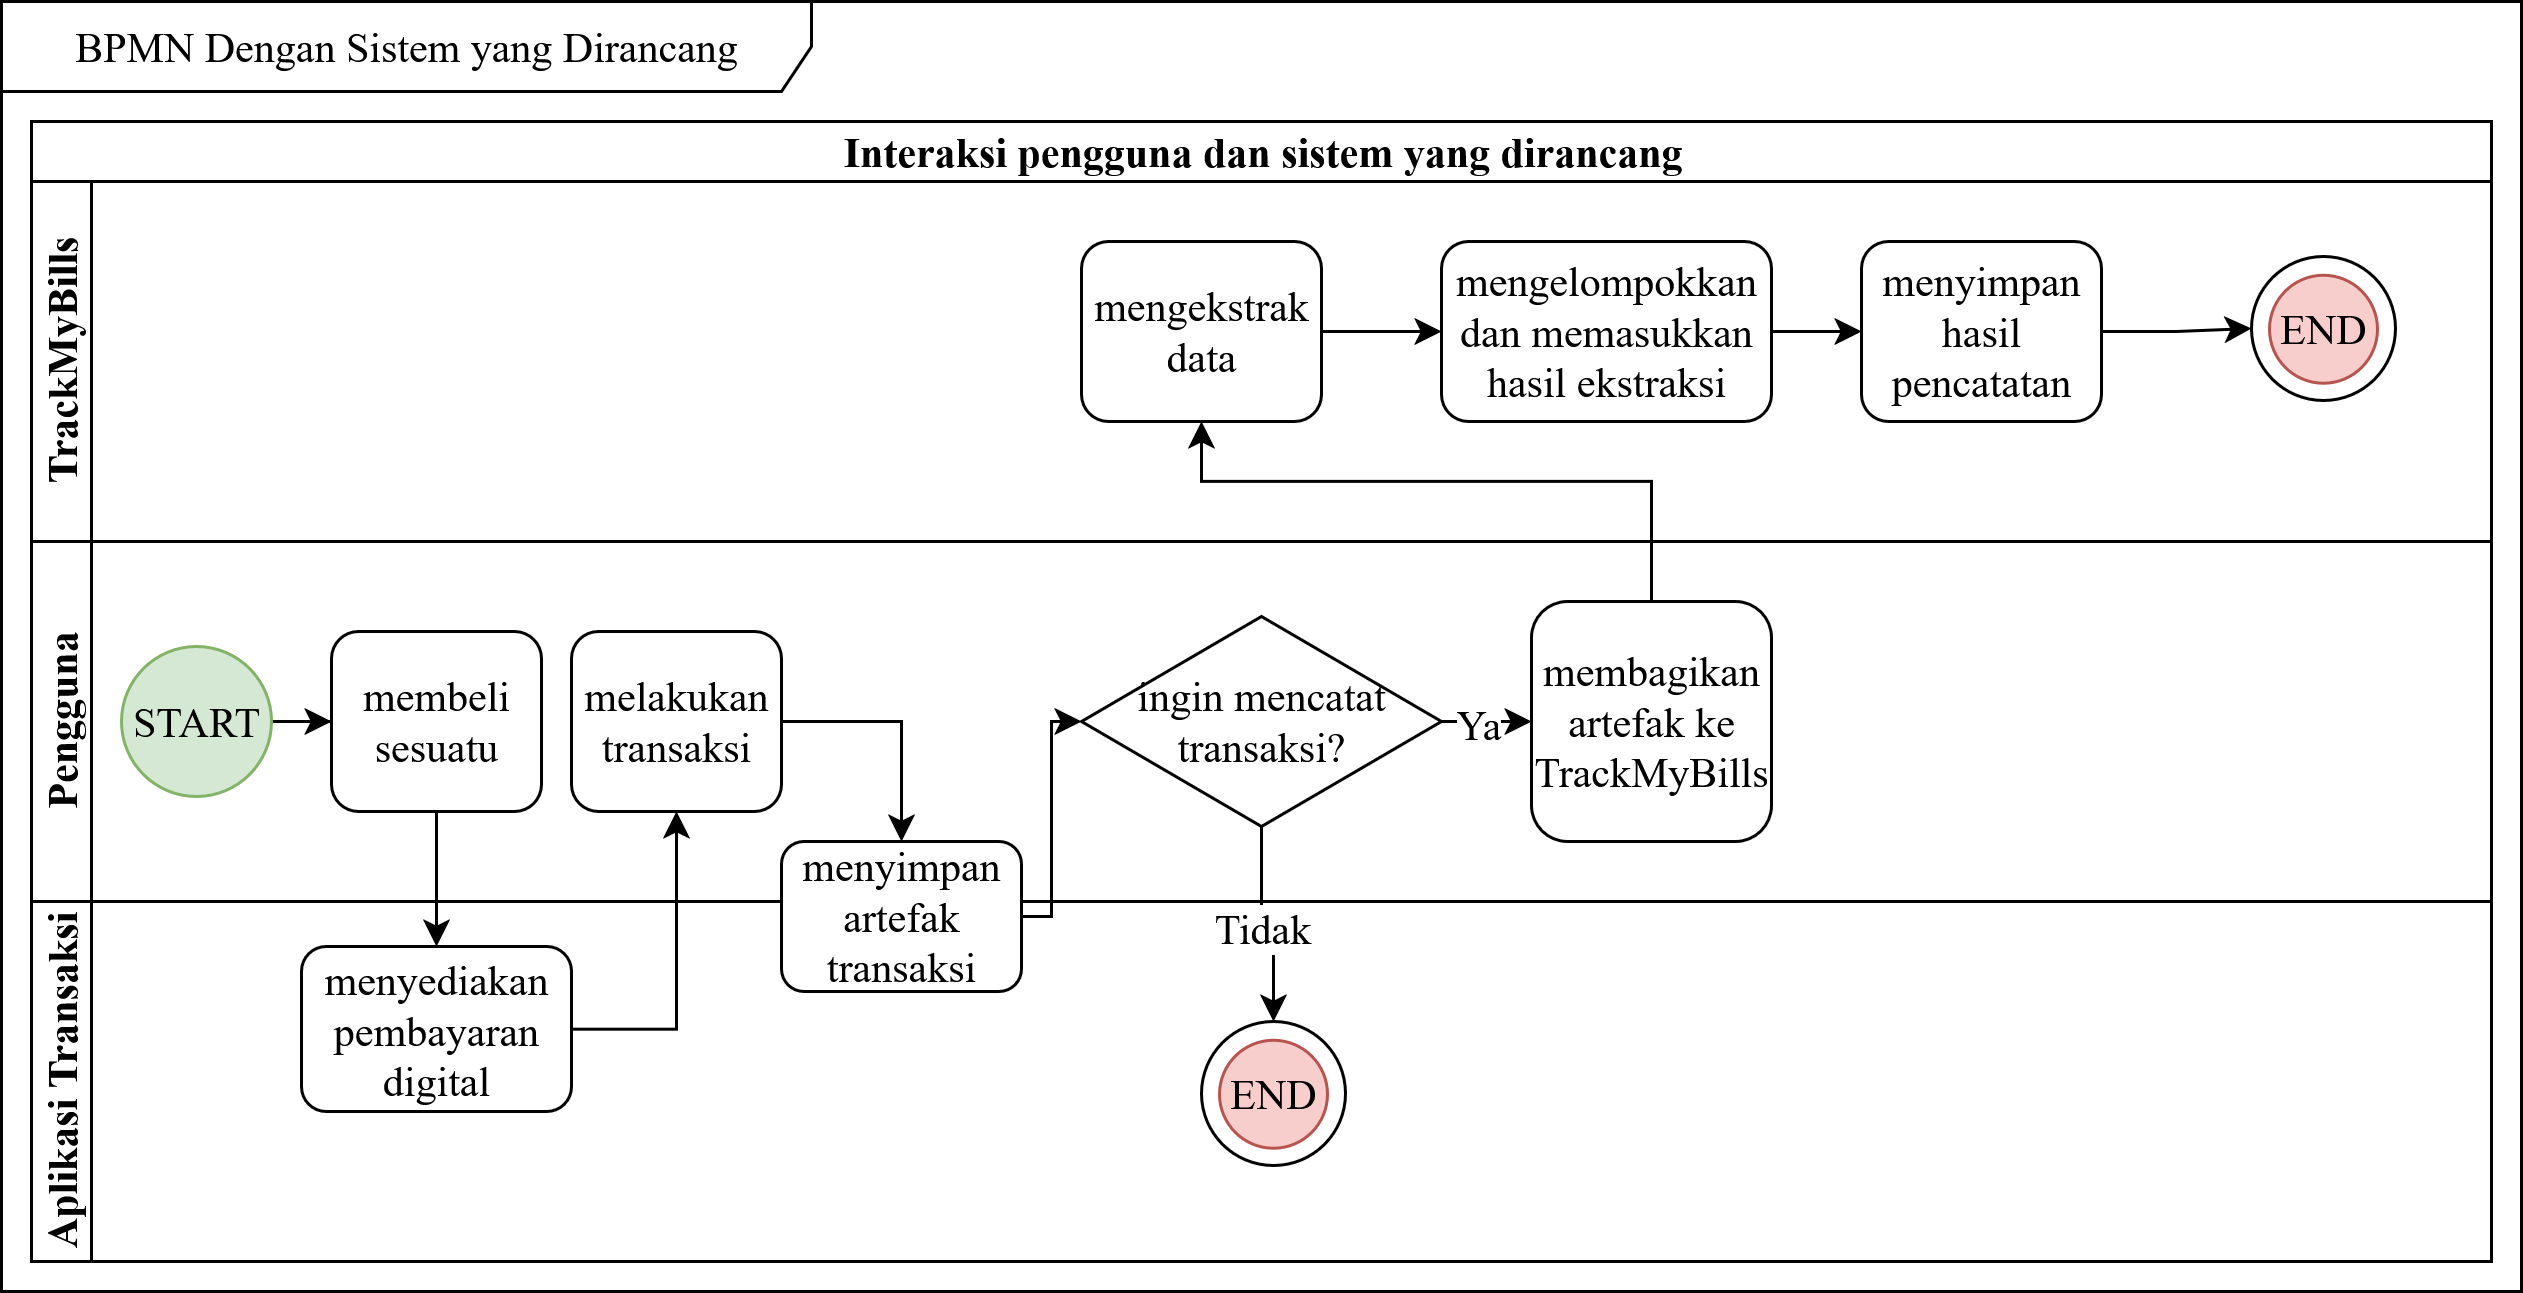
\includegraphics[width=1\textwidth]{images/To-be.png}
    \caption{BPMN untuk \emph{use case} utama sistem (\emph{share-extract-save})}
    \label{fig:bpmn-to-be}
\end{figure}

\autoref{fig:use-case-diagram} menunjukkan \emph{use case diagram} sistem pencatatan pengeluaran berbasis \emph{mobile}. Diagram ini menggambarkan interaksi antara pengguna dan sistem pada \emph{use case} yang telah diidentifikasikan dari kebutuhan fungsional. \autoref{tab:use-case-list} menyajikan daftar \emph{use case} yang diidentifikasi dalam sistem beserta kode kebutuhan fungsional yang terkait. \emph{Use case} menunjukkan seluruh kasus penggunaan yang dapat dilakukan pengguna terhadap sistem. 

% \emph{Use case} menunjukkan seluruh kasus penggunaan yang dapat dilakukan pengguna terhadap sistem. Kasus-kasus yang didefinisikan tersebut menjadi dasar untuk mengembangkan fitur-fitur dalam sistem untuk memenuhi kebutuhan fungsional dan kebutuhan non-fungsional pengguna. \emph{Scenarios View} ini bertujuan untuk memberikan gambaran yang jelas tentang bagaimana pengguna akan berinteraksi dengan sistem dan bagaimana sistem akan merespons interaksi tersebut.

\begin{figure}[htbp]
    \centering
    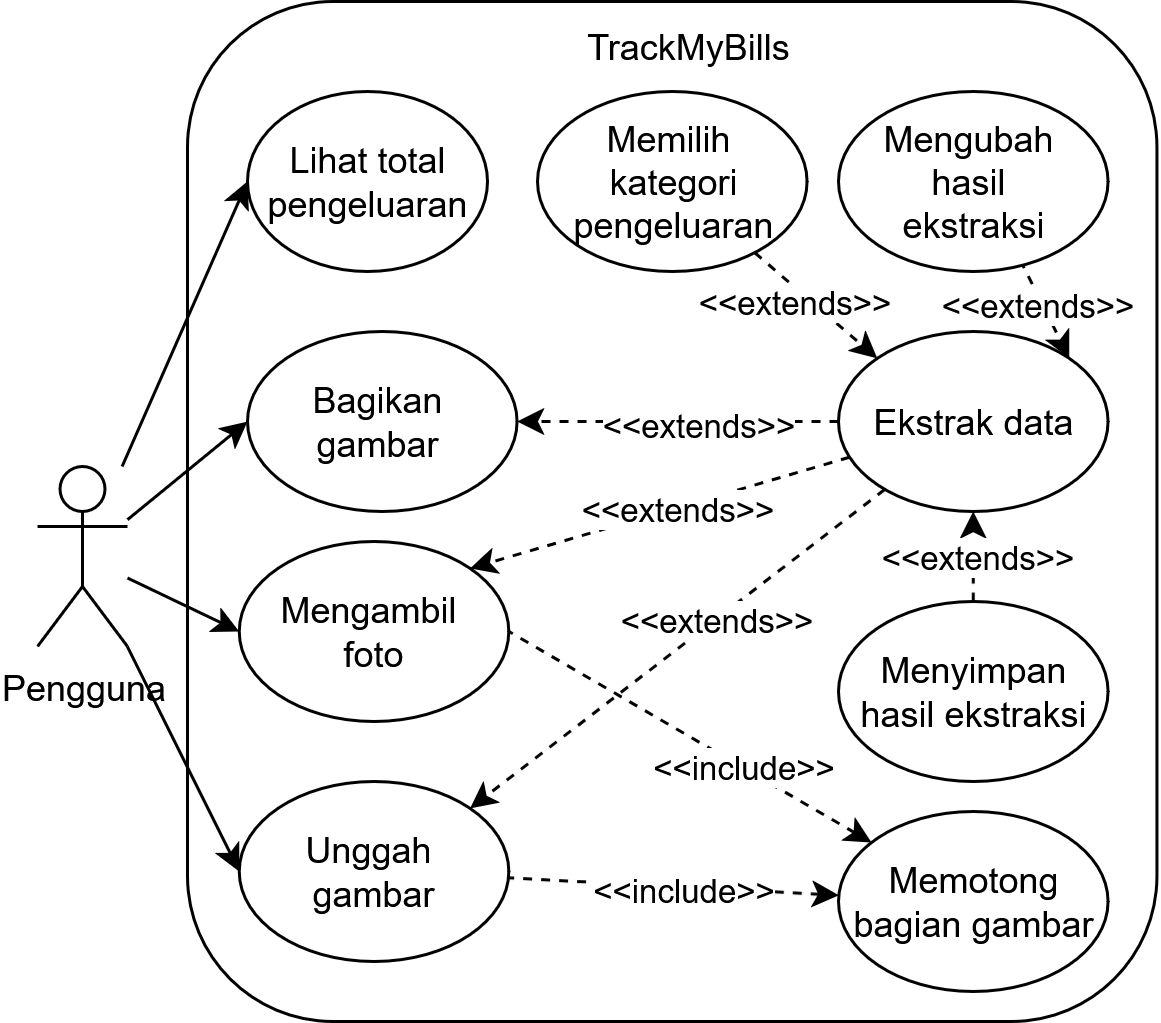
\includegraphics[width=1\textwidth]{images/use-case-diagram.png}
    \caption{\emph{Use case diagram} sistem pencatatan pengeluaran berbasis \emph{mobile}}
    \label{fig:use-case-diagram}
\end{figure}

\begin{table}[h!]
\centering
\caption{Daftar \emph{use case} sistem pencatatan pengeluaran berbasis \emph{mobile}}
\label{tab:use-case-list}
\begin{tabularx}{\textwidth}{|p{1.6cm}|p{1.5cm}|p{2.8cm}|X|}
\hline
\textbf{Kode \emph{Use Case}} & \textbf{Kode FR} & \textbf{\emph{Use Case}} & \textbf{Deskripsi} \\ \hline
UC-01 & FR-01 & Menerima gambar yang dibagikan & Menerima gambar yang dibagikan dari aplikasi eksternal ke sistem \\ \hline
UC-02 & FR-01 & Mengambil foto & Mengakses kamera dari aplikasi dan mengambil foto \\ \hline
UC-03 & FR-01 & Unggah gambar & Memberikan izin mengakses foto dan mengunggah gambar dari galeri \\ \hline
UC-04 & FR-02 & Memotong bagian gambar & Memotong bagian gambar yang diperlukan \\ \hline
UC-05 & FR-03 & Ekstrak data & Mengekstrak data dari gambar yang telah diterima aplikasi \\ \hline
UC-06 & FR-04 & Memilih kategori pengeluaran & Memilih kategori dari data pengeluaran yang diekstrak \\ \hline
UC-07 & FR-04 & Mengubah hasil ekstraksi & Mengubah hasil ekstraksi data sebelum data disimpan \\ \hline
UC-08 & FR-05 & Menyimpan hasil ekstraksi & Menyimpan hasil ekstraksi data dari gambar yang diterima \\ \hline
UC-09 & FR-05 & Lihat total pengeluaran & Melihat total pengeluaran dan pengeluaran per kategori \\ \hline
\end{tabularx}
\end{table}

\newpage